% plan.tex — CPU/memory optimisation of hymeko_core + hymeko_hnn
% Compile: pdflatex plan.tex  (twice, for references)
% NOTE (2026-08-24): no TeX engine on the measurement host; plan.pdf is a
% declared waiver in the report. This source is written to compile as-is.
\documentclass[11pt,a4paper]{article}

\usepackage[margin=25mm]{geometry}
\usepackage{amsmath}
\usepackage{booktabs}
\usepackage{longtable}
\usepackage{tikz}
\usepackage{listings}
\usetikzlibrary{arrows.meta,positioning,fit,backgrounds,calc}
\usepackage[hidelinks]{hyperref}

\title{CPU and Memory Optimisation of \texttt{hymeko\_core} and \texttt{hymeko\_hnn}}
\author{HyMeKo semantic core workspace}
\date{Created-at: 2026-08-24 02:56 CEST}

\begin{document}
\maketitle

\section{Scope and goal}

Measurably reduce CPU time and memory traffic in the sparse-tensor and
hypergraph message-passing hot paths of the \texttt{hymeko/core} workspace,
while preserving:

\begin{itemize}
  \item observable behaviour and numerical results,
  \item public API compatibility,
  \item the existing test suite (17 unit + 106 integration tests).
\end{itemize}

A GPU or FPGA backend may follow later, so the architectural decisions taken
here must not obstruct one. No backend is implemented in this round; the
deliverable on that axis is an interface proposal only.

\paragraph{Estimated time of completion (ETA).}
$\approx$4.5\,h wall, basis: 45\,min benchmark harness authoring
(two bench targets, three workload scales, synthetic generators)
$+$ 40\,min baseline Criterion runs (9 benchmark groups, reduced sample
sizes at the large scale) $+$ 90\,min implementation across five target
areas $+$ 40\,min post-change re-measurement of the affected cells only
(\S\,\emph{cached facts before new runs}) $+$ 35\,min thread-scaling sweep
(1/4/8/16/24) $+$ 40\,min tests, gates, and report.

\section{Baseline (pre-existing, this host)}

\begin{center}
\begin{tabular}{ll}
\toprule
CPU               & Intel Core Ultra 9 275HX, 24 logical cores \\
RAM               & 63.4\,GiB \\
GPU               & NVIDIA RTX 5080 Laptop, 16\,GiB (unused this round) \\
SIMD lexer        & $\approx$6.05\,ms, $\approx$475\,MiB/s \\
parse + interning & $\approx$107\,ms, $\approx$26.9\,MiB/s \\
bench peak WS     & $\approx$69\,MiB \\
\bottomrule
\end{tabular}
\end{center}

\texttt{cargo test --workspace --release}: 17/17 unit, 106 integration
passing, plus one known documented fixture drift
(\texttt{test\_load\_meta\_geometry}: expected 57 nodes, actual 58). That
drift is pre-existing and upstream-parser-caused. It is \textbf{not} to be
treated as a regression from this work, and \textbf{not} to be silenced by
editing the fixture or the assertion.

\section{Affected files}

\subsection*{Core (lockdown: full --- token required)}
\begin{itemize}
  \item \texttt{hymeko\_core/src/tensor/representations/tensor\_csr.rs}
  \item \texttt{hymeko\_core/Cargo.toml} (bench target registration)
\end{itemize}

\subsection*{Non-core}
\begin{itemize}
  \item \texttt{hymeko\_hnn/src/tensor/message\_passing.rs}
  \item \texttt{hymeko\_hnn/src/tensor/conv/hgnn.rs}
  \item \texttt{hymeko\_hnn/src/tensor/conv/signed\_hgnn.rs}
  \item \texttt{hymeko\_hnn/src/tensor/conv/gcn\_clique.rs}
  \item \texttt{hymeko\_hnn/src/tensor/representations/tensor\_csr\_representations.rs}
  \item \texttt{hymeko\_hnn/src/traversal/hypergraphview.rs}
  \item \texttt{hymeko\_hnn/Cargo.toml} (criterion dev-dependency, bench targets)
\end{itemize}

\subsection*{Allowlisted (tests / benches / docs)}
\begin{itemize}
  \item \texttt{hymeko\_core/benches/*}, \texttt{hymeko\_hnn/benches/*}
  \item \texttt{hymeko\_core/tests/test\_tensor\_representations/*}
  \item \texttt{docs/plans/2026-08-24-cpu-optimization/*}, \texttt{reports/*}
  \item \texttt{scripts/dev/*} (thread sweep, peak-memory harness)
\end{itemize}

\section{CORE.YAML items touched}

Not empty. Escalated and approved before implementation:

\begin{quote}
\texttt{APPROVED-CORE-EDIT: csr-spmv-spmm-into}
\end{quote}

quoted verbatim from the user's chat turn of 2026-08-24. It authorises the
\texttt{tensor\_csr.rs} and \texttt{hymeko\_core/Cargo.toml} edits above and
nothing else. The same turn authorised creating this workspace's
\texttt{CORE.YAML} and \texttt{tools.yaml} (previously absent --- a \S1/\S11
\texttt{on\_missing\_file} halt) and approved \texttt{samply} as the
\S10 CPU-profiler substitution for \texttt{cargo flamegraph}, which has no
working backend on Windows.

\section{Interface changes}

All additive. No existing signature changes.

\begin{lstlisting}[basicstyle=\ttfamily\small,breaklines=true]
impl<F: Real> TensorCsr<F> {
    // new, allocation-free
    pub fn spmv_into(&self, x: &[F], y: &mut [F]);
    pub fn spmv_into_serial(&self, x: &[F], y: &mut [F]);
    pub fn spmv_into_parallel(&self, x: &[F], y: &mut [F]);

    pub fn spmm_into(&self, x: &[F], feature_dim: usize, y: &mut [F]);
    pub fn spmm_into_serial(&self, x: &[F], feature_dim: usize, y: &mut [F]);
    pub fn spmm_into_parallel(&self, x: &[F], feature_dim: usize, y: &mut [F]);

    // unchanged signatures; now thin allocating wrappers over *_into
    pub fn spmv(&self, x: &[F]) -> Vec<F>;
    pub fn spmm(&self, x_flat: &[F], feature_dim: usize) -> Vec<F>;
}
\end{lstlisting}

The explicit \texttt{\_serial} / \texttt{\_parallel} pair is deliberate: it
is what makes the ``serial output $\equiv$ parallel output'' regression test
expressible, and it is the seam a later \texttt{CpuSerialBackend} /
\texttt{CpuRayonBackend} split reuses (\S\ref{sec:backend}).

The message-passing layer gains the same treatment --- explicit serial and
parallel entry points behind an auto-dispatching default --- plus fused
variants that remove intermediate buffers.

\section{Optimisation hypotheses}

Stated as hypotheses to be confirmed by measurement, per the
\emph{analyze, don't declare} principle. Each is paired with the
discriminating measurement.

\begin{longtable}{p{0.30\textwidth}p{0.34\textwidth}p{0.28\textwidth}}
\toprule
\textbf{Hypothesis} & \textbf{Mechanism} & \textbf{Discriminating measurement} \\
\midrule
H1: \texttt{spmv}/\texttt{spmm} are output-allocation bound at small sizes
& one \texttt{vec![zero; n]} per call
& \texttt{spmv} vs \texttt{spmv\_into} on a pre-allocated buffer, small scale \\
\addlinespace
H2: CSR ops scale with cores when partitioned by output rows
& rows are disjoint; \texttt{par\_chunks\_mut} needs no synchronisation
& thread sweep 1/4/8/16/24 at each scale \\
\addlinespace
H3: Rayon overhead dominates below some nnz threshold
& fork/join cost exceeds the work
& measure the crossover; set the threshold from it, do not guess \\
\addlinespace
H4: HGNN/Signed-HGNN forward is dominated by \emph{re-traversing} the
incidence structure once per output feature
& the \texttt{for f in 0..d\_out} loop walks all edges each iteration and
allocates 3 temporaries per feature
& feature-blocked single-traversal rewrite; expect gain to grow with
\texttt{d\_out} \\
\addlinespace
H5: scatter can be parallelised with no atomics
& the node-first incidence CSR makes each node's output independently
computable
& serial vs parallel bitwise equality test + thread sweep \\
\addlinespace
H6: \texttt{HyperGraphView::from\_ir} is sort-bound
& two comparison sorts over the triple array
& profile with samply before touching it \\
\bottomrule
\end{longtable}

\paragraph{Bitwise-identity argument for H5.}
Both incidence CSRs are built from the same triple multiset. The edge-first
array is sorted by $(e,n)$; the node-first array by $(n,e)$. Today's scatter
iterates $e = 0 \ldots m-1$ and, for each, accumulates into $y[v]$; a given
node $v$ therefore receives its contributions in strictly increasing edge
order. The node-first traversal visits, for each $v$, exactly that node's
incidences in strictly increasing edge order as well. The summation order per
output element is thus \emph{identical}, not merely equivalent --- so the
rewrite is bitwise reproducible, and parallelising over nodes introduces no
reassociation. The same argument covers \texttt{clique\_diag}. This is
asserted by test, not by assumption.

\section{Test strategy}

\begin{description}
  \item[Unit / correctness (new, in \texttt{hymeko\_core/tests/})]
    \texttt{spmv} vs a dense reference; \texttt{spmm} vs a dense reference
    across \texttt{feature\_dim} $\in \{1,8,32,128\}$; serial vs parallel
    bitwise equality for every new kernel; gather/scatter vs the manual
    $B^\top x$ / $Bx_e$ references; the implicit clique pipeline vs its
    explicit three-step form; HGNN and Signed-HGNN forward vs a
    pre-refactor reference implementation retained in the test file.
  \item[Degenerate shapes] empty (0 rows, 0 nnz), singleton (1 row / 1 node
    / 1 edge), empty rows interleaved with dense ones, and irregular degree
    distributions (power-law-ish edge cardinalities).
  \item[Regression] each behaviour-preserving rewrite ships a test that
    would fail against a naive reordering of the accumulation --- i.e. the
    bitwise-equality assertions, not merely tolerance assertions.
  \item[Existing suite] \texttt{cargo test --workspace --release} must stay
    at 17 unit / 106 integration passing, with the 57/58 drift reported
    separately and untouched.
  \item[Gates] \texttt{cargo fmt --all -- --check};
    \texttt{cargo clippy --workspace --all-targets -- -D warnings}.
\end{description}

\section{Performance budget}

\begin{itemize}
  \item Peak working set for the benchmark process: $\le$1\,GiB at the large
    workload scale; far under the 16\,GB \S4 cap, which is observed and
    asserted on Windows rather than cgroup-enforced.
  \item No regression $>$10\,\% on any measured cell versus the recorded
    baseline (\S3 regression discipline). A regression above that blocks
    completion until profiled; the default attribution is ``a bug was
    introduced''.
  \item Any speedup claim $>$10\,\% must be backed by a samply profile
    showing the cost moved out of the targeted site --- not by wall-clock
    variance.
  \item Small-scale latency must not regress: the parallel path is gated
    behind a measured threshold precisely so the small case stays serial.
\end{itemize}

\section{Measurement protocol}

Criterion, with \texttt{black\_box} on every input, \texttt{Throughput}
declared per group (elements $=$ nnz for SpMV, nnz $\times$
\texttt{feature\_dim} for SpMM, incidences for gather/scatter), and setup
and allocation hoisted out of the timed closure via
\texttt{iter\_batched\_ref} except in the construction/allocation benchmarks
where allocation \emph{is} the subject.

Workloads are deterministic (fixed-seed LCG, no system entropy) at three
scales: \textbf{small} (latency and parallel-overhead regime),
\textbf{medium}, \textbf{large} (throughput and memory-bandwidth regime).

Baselines are saved with \texttt{--save-baseline before} and compared with
\texttt{--baseline before}; medians and Criterion confidence intervals are
what get reported, not single shots. Thread scaling is driven by
\texttt{RAYON\_NUM\_THREADS} $\in \{1,4,8,16,24\}$ through a documented
script. Build configurations compared: default release versus
\texttt{RUSTFLAGS="-C target-cpu=native"}; \texttt{lto = "thin"} with
\texttt{codegen-units = 1} measured but recommended as default only if it
demonstrates a real gain.

\section{Rollback path}

The working tree is clean at \texttt{45b0512} on \texttt{main}. Every change
is additive or a body rewrite behind an unchanged signature, so rollback is
\texttt{git checkout -- <file>} per file, or \texttt{git reset --hard
45b0512} for the whole task. The new \texttt{*\_into} API is additive: if a
parallel kernel is withdrawn, its \texttt{\_serial} sibling remains a
complete implementation and the dispatcher can be pinned to it by lowering
the threshold to \texttt{usize::MAX}. Criterion baselines are kept under
\texttt{target/criterion/} so a withdrawn change can be re-measured against
the same recorded \texttt{before}.

\section{Risk anticipation}

\begin{description}
  \item[Performance-contract preservation.] The existing kernels carry an
    implicit contract that output is fully overwritten (\texttt{spmv}
    allocates a zeroed vector; \texttt{scatter\_nodes\_from\_edges} explicitly
    zeroes its output first). The new \texttt{\_into} forms must preserve
    ``fully overwritten, not accumulated'' --- a caller passing a dirty
    buffer must get the same result as one passing a fresh zeroed one. This
    is the highest-risk case flagged by \S2: a new branch beside an existing
    one must inherit every contract the old branch enforced. Tested
    explicitly by passing a poisoned (non-zero sentinel) output buffer.
  \item[Worst-case input.] Large scale: $\approx$500k rows,
    $\approx$8M nnz for CSR; $\approx$200k nodes / $\approx$100k edges /
    $\approx$2M incidences for the hypergraph, with irregular edge
    cardinality. That is the shape the thresholds and the memory budget are
    chosen against, not the toy fixture.
  \item[Floating-point drift.] The stated goal is bitwise identity wherever
    the accumulation order argument holds. Where it cannot hold, the change
    is not made. No Kahan/Neumaier reformulation is introduced in this round
    --- that would itself change results.
  \item[False speedup from a cold-vs-warm allocator.] Comparing an
    allocating API against an \texttt{\_into} API can flatter the latter if
    the buffer is allocated once outside the loop while the baseline
    allocates every iteration --- which is exactly the real difference, but
    it must be reported as ``allocation removed'', not as ``kernel faster''.
    The two are separated in the report.
  \item[Thread-count contamination.] Rayon's global pool is process-wide;
    a sweep must set \texttt{RAYON\_NUM\_THREADS} per process invocation,
    not per benchmark group.
  \item[Empty plan dir hygiene.] If this task is abandoned, delete
    \texttt{docs/plans/2026-08-24-cpu-optimization/}.
\end{description}

\section{Backend-neutral boundary (proposal only)}
\label{sec:backend}

No GPU or FPGA backend is implemented in this round. The design constraint
is that the abstraction must cost \emph{nothing} on the current CPU hot path.

The recommendation is a \textbf{static, generic backend trait} selecting
kernels at compile time, not a \texttt{Box<dyn Backend>}:

\begin{itemize}
  \item \emph{trait + generic dispatch} --- monomorphised, inlinable, zero
    runtime cost; the hot loop keeps its current codegen. Preferred.
  \item \emph{enum dispatch} --- one predictable branch per \emph{call}, not
    per element; acceptable at the layer boundary (a whole SpMM), unacceptable
    inside a kernel. Reasonable for a runtime-selected device.
  \item \emph{feature-gated modules} --- needed anyway for CUDA/FPGA toolchain
    isolation, but insufficient alone: it cannot express runtime device
    selection.
\end{itemize}

The proposed shape is generic dispatch for the CPU tiers
(\texttt{CpuSerialBackend}, \texttt{CpuRayonBackend}) with an enum facade at
the outermost call site for device selection, and \texttt{cuda}/\texttt{fpga}
feature gates around the device modules. The \texttt{*\_into} signatures
introduced here are already the right shape for it: explicit output buffers,
no hidden allocation, no ownership transfer --- which is what a device
backend needs in order to write into pinned or device-resident memory.
Details in the report.

\section{Diagrams}

Architecture and dataflow: \texttt{plan.tikz} (TikZ, \verb|\input|-able).
Sequence and dependency views: \texttt{plan.mmd} (Mermaid).

% plan.tikz — architecture / dataflow / module boundaries
% % plan.tikz — architecture / dataflow / module boundaries
% % plan.tikz — architecture / dataflow / module boundaries
% \input{plan.tikz} from plan.tex, or compile standalone by wrapping in
% a minimal document with \usepackage{tikz} and the libraries below:
%   \usetikzlibrary{arrows.meta,positioning,fit,backgrounds,calc}

\begin{figure}[htbp]
\centering
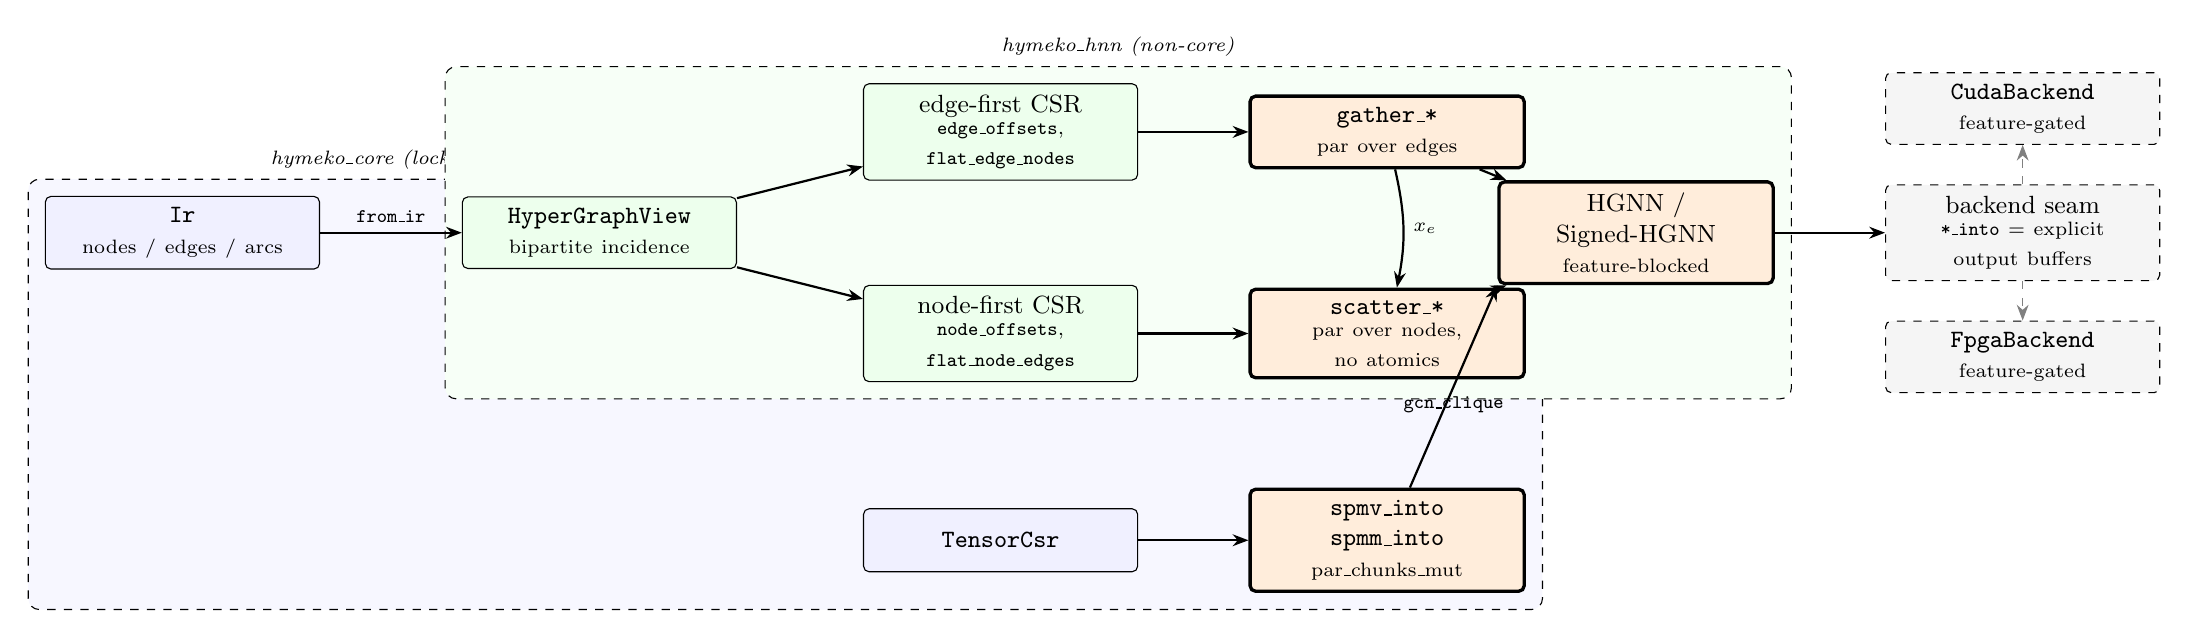
\begin{tikzpicture}[
  font=\small,
  node distance=6mm and 10mm,
  box/.style={draw, rounded corners=2pt, align=center, inner sep=4pt,
              minimum height=8mm, text width=32mm},
  core/.style={box, fill=blue!6},
  hnn/.style={box, fill=green!7},
  newk/.style={box, fill=orange!14, very thick},
  future/.style={box, fill=gray!8, dashed},
  flow/.style={-{Stealth[length=2mm]}, thick},
  weak/.style={-{Stealth[length=2mm]}, dashed, gray}
]

% ---- data sources -------------------------------------------------
\node[core] (ir) {\texttt{Ir}\\{\scriptsize nodes / edges / arcs}};
\node[hnn, right=18mm of ir] (view) {\texttt{HyperGraphView}\\{\scriptsize bipartite incidence}};

% ---- the two incidence CSRs (the load-bearing detail) -------------
\node[hnn, above right=2mm and 16mm of view] (ecsr)
  {edge-first CSR\\{\scriptsize \texttt{edge\_offsets},\\\texttt{flat\_edge\_nodes}}};
\node[hnn, below right=2mm and 16mm of view] (ncsr)
  {node-first CSR\\{\scriptsize \texttt{node\_offsets},\\\texttt{flat\_node\_edges}}};

\draw[flow] (ir) -- node[above,font=\scriptsize] {\texttt{from\_ir}} (view);
\draw[flow] (view) -- (ecsr);
\draw[flow] (view) -- (ncsr);

% ---- kernels ------------------------------------------------------
\node[newk, right=14mm of ecsr] (gather) {\texttt{gather\_*}\\{\scriptsize par over edges}};
\node[newk, right=14mm of ncsr] (scatter) {\texttt{scatter\_*}\\{\scriptsize par over nodes,\\no atomics}};

\draw[flow] (ecsr) -- (gather);
\draw[flow] (ncsr) -- (scatter);
\draw[flow] (gather) to[bend left=12] node[right,font=\scriptsize] {$x_e$} (scatter);

% ---- convolution layer -------------------------------------------
\node[newk, right=14mm of $(gather)!0.5!(scatter)$] (conv)
  {HGNN / Signed-HGNN\\{\scriptsize feature-blocked}};
\draw[flow] (gather) -- (conv);
\draw[flow] (scatter) -- (conv);

% ---- CSR primitive path -------------------------------------------
\node[core, below=16mm of ncsr] (csr) {\texttt{TensorCsr}};
\node[newk, right=14mm of csr] (spmm)
  {\texttt{spmv\_into}\\\texttt{spmm\_into}\\{\scriptsize par\_chunks\_mut}};
\draw[flow] (csr) -- (spmm);
\draw[flow] (spmm) -- node[below,font=\scriptsize] {\texttt{gcn\_clique}} (conv.south west);

% ---- future backends ----------------------------------------------
\node[future, right=14mm of conv] (be) {backend seam\\{\scriptsize \texttt{*\_into} = explicit\\output buffers}};
\node[future, above=5mm of be] (cuda) {\texttt{CudaBackend}\\{\scriptsize feature-gated}};
\node[future, below=5mm of be] (fpga) {\texttt{FpgaBackend}\\{\scriptsize feature-gated}};
\draw[flow] (conv) -- (be);
\draw[weak] (be) -- (cuda);
\draw[weak] (be) -- (fpga);

% ---- crate boundary ------------------------------------------------
\begin{scope}[on background layer]
  \node[draw, dashed, fill=blue!3, inner sep=6pt, rounded corners,
        fit=(ir)(csr)(spmm), label={[font=\scriptsize\itshape]above left:hymeko\_core (lockdown: full)}] {};
  \node[draw, dashed, fill=green!3, inner sep=6pt, rounded corners,
        fit=(view)(ecsr)(ncsr)(gather)(scatter)(conv), label={[font=\scriptsize\itshape]above:hymeko\_hnn (non-core)}] {};
\end{scope}

\end{tikzpicture}
\caption{Dataflow and module boundaries. Orange nodes are the kernels this
plan rewrites. The load-bearing structural fact is that
\texttt{HyperGraphView} already materialises \emph{both} incidence
orientations from the same triple multiset: gather is naturally parallel over
edges on the edge-first CSR, and scatter becomes naturally parallel over
\emph{nodes} on the node-first CSR --- with per-element summation order
unchanged, hence no atomics, no locks, and bitwise-identical output. The
\texttt{*\_into} signatures (explicit caller-owned output buffers) are also
the seam a later device backend needs.}
\end{figure}

\begin{figure}[htbp]
\centering
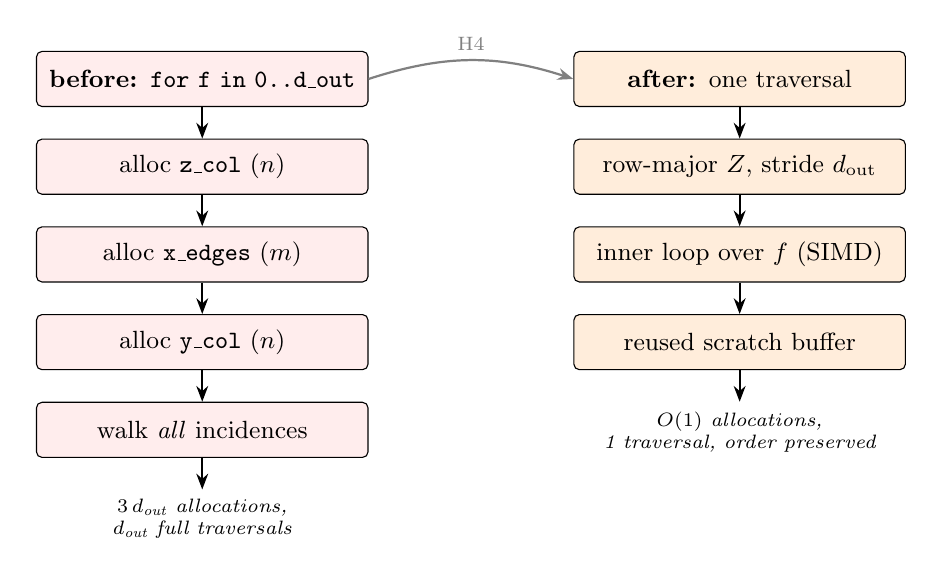
\begin{tikzpicture}[
  font=\small,
  box/.style={draw, rounded corners=2pt, align=center, inner sep=3pt,
              minimum height=7mm, text width=40mm},
  old/.style={box, fill=red!7},
  new/.style={box, fill=orange!14},
  flow/.style={-{Stealth[length=2mm]}, thick},
  node distance=4mm
]

\node[old] (o1) {\textbf{before:} \texttt{for f in 0..d\_out}};
\node[old, below=of o1] (o2) {alloc \texttt{z\_col} ($n$)};
\node[old, below=of o2] (o3) {alloc \texttt{x\_edges} ($m$)};
\node[old, below=of o3] (o4) {alloc \texttt{y\_col} ($n$)};
\node[old, below=of o4] (o5) {walk \emph{all} incidences};
\node[below=of o5, font=\scriptsize\itshape, text width=42mm, align=center]
  (o6) {$3\,d_{\text{out}}$ allocations,\\$d_{\text{out}}$ full traversals};

\draw[flow] (o1) -- (o2); \draw[flow] (o2) -- (o3);
\draw[flow] (o3) -- (o4); \draw[flow] (o4) -- (o5);
\draw[flow] (o5) -- (o6);

\node[new, right=26mm of o1] (n1) {\textbf{after:} one traversal};
\node[new, below=of n1] (n2) {row-major $Z$, stride $d_{\text{out}}$};
\node[new, below=of n2] (n3) {inner loop over $f$ (SIMD)};
\node[new, below=of n3] (n4) {reused scratch buffer};
\node[below=of n4, font=\scriptsize\itshape, text width=42mm, align=center]
  (n5) {$O(1)$ allocations,\\1 traversal, order preserved};

\draw[flow] (n1) -- (n2); \draw[flow] (n2) -- (n3);
\draw[flow] (n3) -- (n4); \draw[flow] (n4) -- (n5);

\draw[flow, gray] (o1.east) to[bend left=18] node[above,font=\scriptsize]{H4} (n1.west);

\end{tikzpicture}
\caption{Hypothesis H4: the convolution forward passes re-walk the entire
incidence structure once per output feature and allocate three temporaries
each time. Blocking the feature loop \emph{inside} the traversal keeps the
per-element summation order (and hence the numerics) but turns
$d_{\text{out}}$ traversals into one. The expected gain grows with
$d_{\text{out}}$ --- which is what the \texttt{feature\_dim} $\in
\{1,8,32,128\}$ sweep is designed to confirm or refute.}
\end{figure}
 from plan.tex, or compile standalone by wrapping in
% a minimal document with \usepackage{tikz} and the libraries below:
%   \usetikzlibrary{arrows.meta,positioning,fit,backgrounds,calc}

\begin{figure}[htbp]
\centering
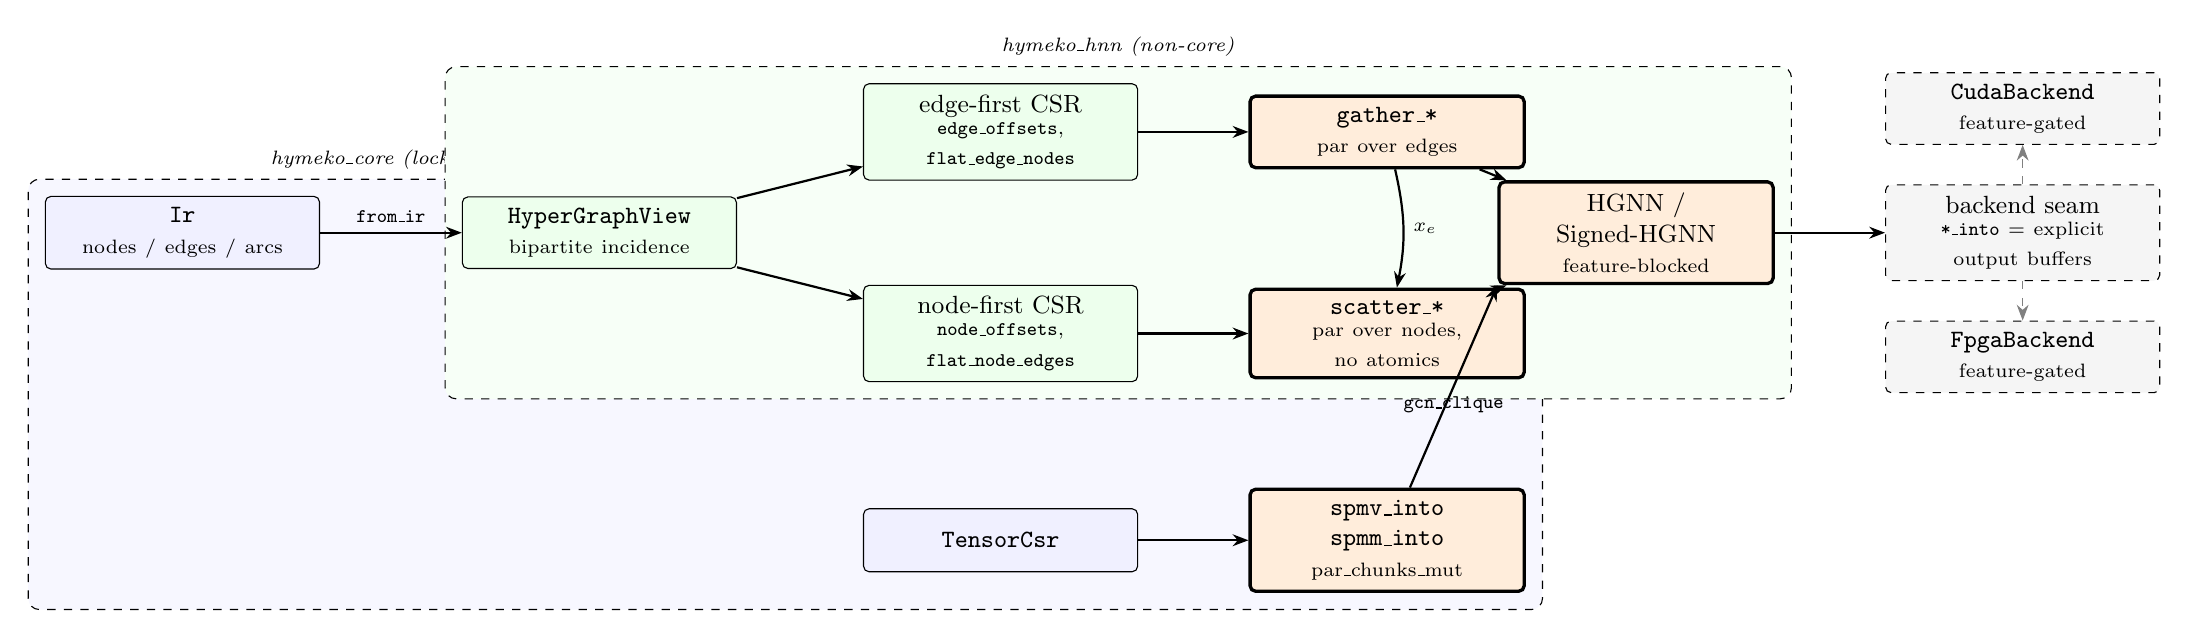
\begin{tikzpicture}[
  font=\small,
  node distance=6mm and 10mm,
  box/.style={draw, rounded corners=2pt, align=center, inner sep=4pt,
              minimum height=8mm, text width=32mm},
  core/.style={box, fill=blue!6},
  hnn/.style={box, fill=green!7},
  newk/.style={box, fill=orange!14, very thick},
  future/.style={box, fill=gray!8, dashed},
  flow/.style={-{Stealth[length=2mm]}, thick},
  weak/.style={-{Stealth[length=2mm]}, dashed, gray}
]

% ---- data sources -------------------------------------------------
\node[core] (ir) {\texttt{Ir}\\{\scriptsize nodes / edges / arcs}};
\node[hnn, right=18mm of ir] (view) {\texttt{HyperGraphView}\\{\scriptsize bipartite incidence}};

% ---- the two incidence CSRs (the load-bearing detail) -------------
\node[hnn, above right=2mm and 16mm of view] (ecsr)
  {edge-first CSR\\{\scriptsize \texttt{edge\_offsets},\\\texttt{flat\_edge\_nodes}}};
\node[hnn, below right=2mm and 16mm of view] (ncsr)
  {node-first CSR\\{\scriptsize \texttt{node\_offsets},\\\texttt{flat\_node\_edges}}};

\draw[flow] (ir) -- node[above,font=\scriptsize] {\texttt{from\_ir}} (view);
\draw[flow] (view) -- (ecsr);
\draw[flow] (view) -- (ncsr);

% ---- kernels ------------------------------------------------------
\node[newk, right=14mm of ecsr] (gather) {\texttt{gather\_*}\\{\scriptsize par over edges}};
\node[newk, right=14mm of ncsr] (scatter) {\texttt{scatter\_*}\\{\scriptsize par over nodes,\\no atomics}};

\draw[flow] (ecsr) -- (gather);
\draw[flow] (ncsr) -- (scatter);
\draw[flow] (gather) to[bend left=12] node[right,font=\scriptsize] {$x_e$} (scatter);

% ---- convolution layer -------------------------------------------
\node[newk, right=14mm of $(gather)!0.5!(scatter)$] (conv)
  {HGNN / Signed-HGNN\\{\scriptsize feature-blocked}};
\draw[flow] (gather) -- (conv);
\draw[flow] (scatter) -- (conv);

% ---- CSR primitive path -------------------------------------------
\node[core, below=16mm of ncsr] (csr) {\texttt{TensorCsr}};
\node[newk, right=14mm of csr] (spmm)
  {\texttt{spmv\_into}\\\texttt{spmm\_into}\\{\scriptsize par\_chunks\_mut}};
\draw[flow] (csr) -- (spmm);
\draw[flow] (spmm) -- node[below,font=\scriptsize] {\texttt{gcn\_clique}} (conv.south west);

% ---- future backends ----------------------------------------------
\node[future, right=14mm of conv] (be) {backend seam\\{\scriptsize \texttt{*\_into} = explicit\\output buffers}};
\node[future, above=5mm of be] (cuda) {\texttt{CudaBackend}\\{\scriptsize feature-gated}};
\node[future, below=5mm of be] (fpga) {\texttt{FpgaBackend}\\{\scriptsize feature-gated}};
\draw[flow] (conv) -- (be);
\draw[weak] (be) -- (cuda);
\draw[weak] (be) -- (fpga);

% ---- crate boundary ------------------------------------------------
\begin{scope}[on background layer]
  \node[draw, dashed, fill=blue!3, inner sep=6pt, rounded corners,
        fit=(ir)(csr)(spmm), label={[font=\scriptsize\itshape]above left:hymeko\_core (lockdown: full)}] {};
  \node[draw, dashed, fill=green!3, inner sep=6pt, rounded corners,
        fit=(view)(ecsr)(ncsr)(gather)(scatter)(conv), label={[font=\scriptsize\itshape]above:hymeko\_hnn (non-core)}] {};
\end{scope}

\end{tikzpicture}
\caption{Dataflow and module boundaries. Orange nodes are the kernels this
plan rewrites. The load-bearing structural fact is that
\texttt{HyperGraphView} already materialises \emph{both} incidence
orientations from the same triple multiset: gather is naturally parallel over
edges on the edge-first CSR, and scatter becomes naturally parallel over
\emph{nodes} on the node-first CSR --- with per-element summation order
unchanged, hence no atomics, no locks, and bitwise-identical output. The
\texttt{*\_into} signatures (explicit caller-owned output buffers) are also
the seam a later device backend needs.}
\end{figure}

\begin{figure}[htbp]
\centering
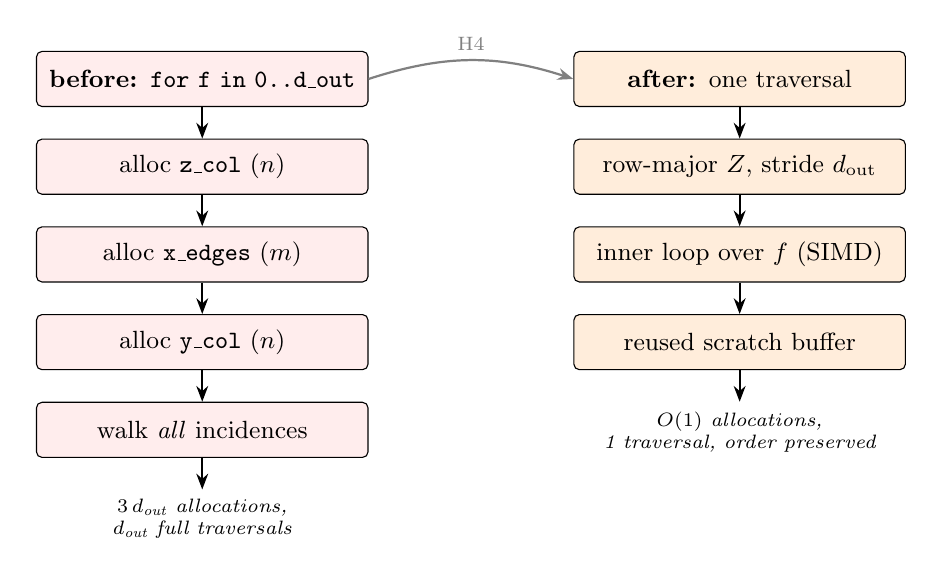
\begin{tikzpicture}[
  font=\small,
  box/.style={draw, rounded corners=2pt, align=center, inner sep=3pt,
              minimum height=7mm, text width=40mm},
  old/.style={box, fill=red!7},
  new/.style={box, fill=orange!14},
  flow/.style={-{Stealth[length=2mm]}, thick},
  node distance=4mm
]

\node[old] (o1) {\textbf{before:} \texttt{for f in 0..d\_out}};
\node[old, below=of o1] (o2) {alloc \texttt{z\_col} ($n$)};
\node[old, below=of o2] (o3) {alloc \texttt{x\_edges} ($m$)};
\node[old, below=of o3] (o4) {alloc \texttt{y\_col} ($n$)};
\node[old, below=of o4] (o5) {walk \emph{all} incidences};
\node[below=of o5, font=\scriptsize\itshape, text width=42mm, align=center]
  (o6) {$3\,d_{\text{out}}$ allocations,\\$d_{\text{out}}$ full traversals};

\draw[flow] (o1) -- (o2); \draw[flow] (o2) -- (o3);
\draw[flow] (o3) -- (o4); \draw[flow] (o4) -- (o5);
\draw[flow] (o5) -- (o6);

\node[new, right=26mm of o1] (n1) {\textbf{after:} one traversal};
\node[new, below=of n1] (n2) {row-major $Z$, stride $d_{\text{out}}$};
\node[new, below=of n2] (n3) {inner loop over $f$ (SIMD)};
\node[new, below=of n3] (n4) {reused scratch buffer};
\node[below=of n4, font=\scriptsize\itshape, text width=42mm, align=center]
  (n5) {$O(1)$ allocations,\\1 traversal, order preserved};

\draw[flow] (n1) -- (n2); \draw[flow] (n2) -- (n3);
\draw[flow] (n3) -- (n4); \draw[flow] (n4) -- (n5);

\draw[flow, gray] (o1.east) to[bend left=18] node[above,font=\scriptsize]{H4} (n1.west);

\end{tikzpicture}
\caption{Hypothesis H4: the convolution forward passes re-walk the entire
incidence structure once per output feature and allocate three temporaries
each time. Blocking the feature loop \emph{inside} the traversal keeps the
per-element summation order (and hence the numerics) but turns
$d_{\text{out}}$ traversals into one. The expected gain grows with
$d_{\text{out}}$ --- which is what the \texttt{feature\_dim} $\in
\{1,8,32,128\}$ sweep is designed to confirm or refute.}
\end{figure}
 from plan.tex, or compile standalone by wrapping in
% a minimal document with \usepackage{tikz} and the libraries below:
%   \usetikzlibrary{arrows.meta,positioning,fit,backgrounds,calc}

\begin{figure}[htbp]
\centering
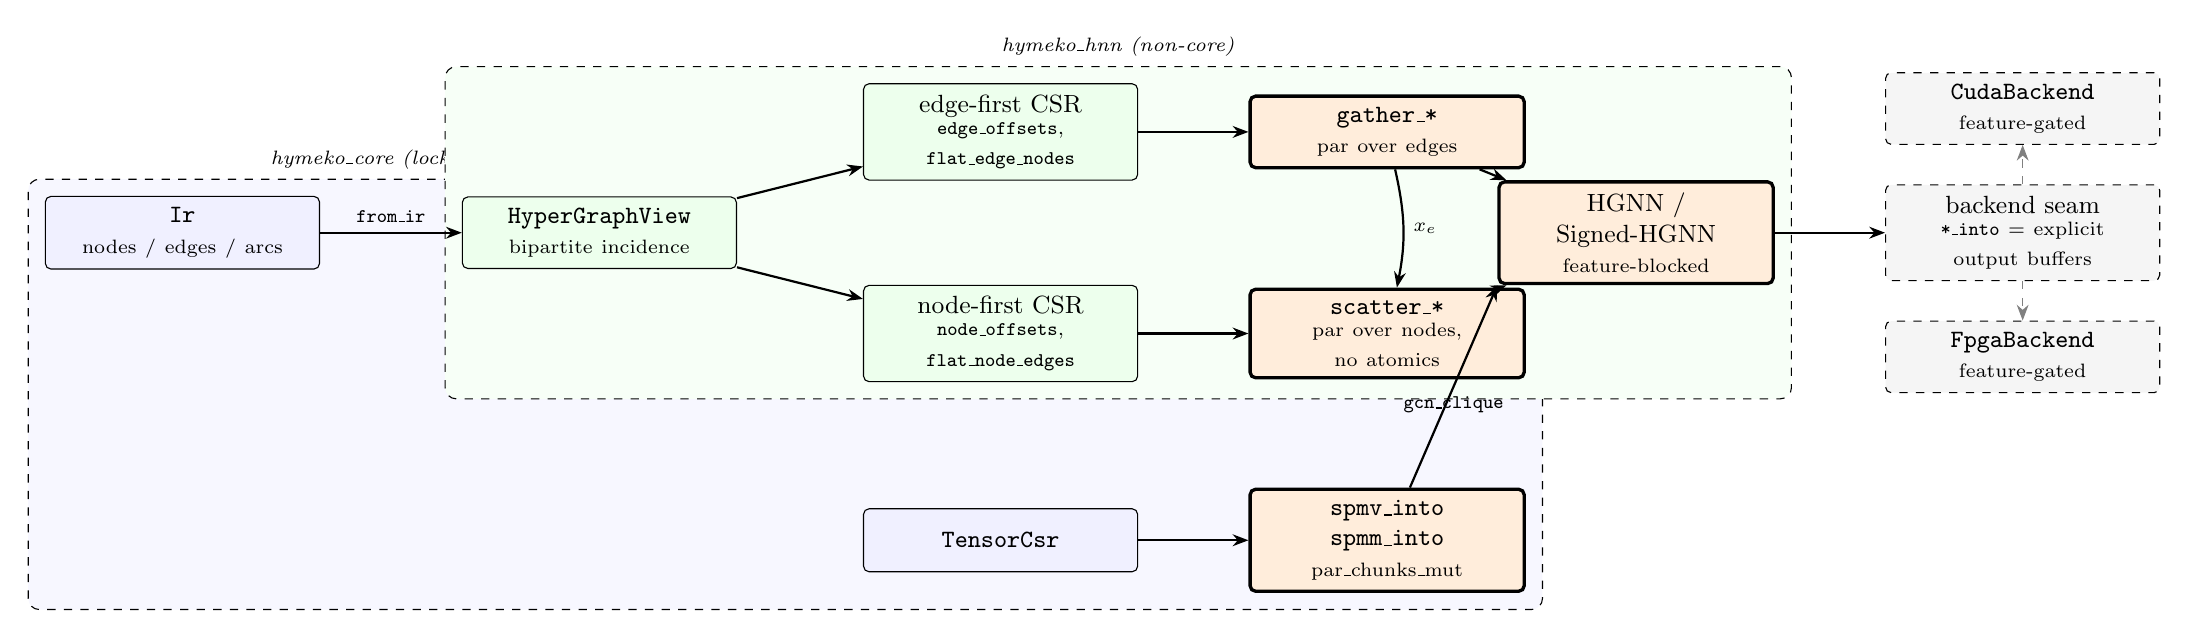
\begin{tikzpicture}[
  font=\small,
  node distance=6mm and 10mm,
  box/.style={draw, rounded corners=2pt, align=center, inner sep=4pt,
              minimum height=8mm, text width=32mm},
  core/.style={box, fill=blue!6},
  hnn/.style={box, fill=green!7},
  newk/.style={box, fill=orange!14, very thick},
  future/.style={box, fill=gray!8, dashed},
  flow/.style={-{Stealth[length=2mm]}, thick},
  weak/.style={-{Stealth[length=2mm]}, dashed, gray}
]

% ---- data sources -------------------------------------------------
\node[core] (ir) {\texttt{Ir}\\{\scriptsize nodes / edges / arcs}};
\node[hnn, right=18mm of ir] (view) {\texttt{HyperGraphView}\\{\scriptsize bipartite incidence}};

% ---- the two incidence CSRs (the load-bearing detail) -------------
\node[hnn, above right=2mm and 16mm of view] (ecsr)
  {edge-first CSR\\{\scriptsize \texttt{edge\_offsets},\\\texttt{flat\_edge\_nodes}}};
\node[hnn, below right=2mm and 16mm of view] (ncsr)
  {node-first CSR\\{\scriptsize \texttt{node\_offsets},\\\texttt{flat\_node\_edges}}};

\draw[flow] (ir) -- node[above,font=\scriptsize] {\texttt{from\_ir}} (view);
\draw[flow] (view) -- (ecsr);
\draw[flow] (view) -- (ncsr);

% ---- kernels ------------------------------------------------------
\node[newk, right=14mm of ecsr] (gather) {\texttt{gather\_*}\\{\scriptsize par over edges}};
\node[newk, right=14mm of ncsr] (scatter) {\texttt{scatter\_*}\\{\scriptsize par over nodes,\\no atomics}};

\draw[flow] (ecsr) -- (gather);
\draw[flow] (ncsr) -- (scatter);
\draw[flow] (gather) to[bend left=12] node[right,font=\scriptsize] {$x_e$} (scatter);

% ---- convolution layer -------------------------------------------
\node[newk, right=14mm of $(gather)!0.5!(scatter)$] (conv)
  {HGNN / Signed-HGNN\\{\scriptsize feature-blocked}};
\draw[flow] (gather) -- (conv);
\draw[flow] (scatter) -- (conv);

% ---- CSR primitive path -------------------------------------------
\node[core, below=16mm of ncsr] (csr) {\texttt{TensorCsr}};
\node[newk, right=14mm of csr] (spmm)
  {\texttt{spmv\_into}\\\texttt{spmm\_into}\\{\scriptsize par\_chunks\_mut}};
\draw[flow] (csr) -- (spmm);
\draw[flow] (spmm) -- node[below,font=\scriptsize] {\texttt{gcn\_clique}} (conv.south west);

% ---- future backends ----------------------------------------------
\node[future, right=14mm of conv] (be) {backend seam\\{\scriptsize \texttt{*\_into} = explicit\\output buffers}};
\node[future, above=5mm of be] (cuda) {\texttt{CudaBackend}\\{\scriptsize feature-gated}};
\node[future, below=5mm of be] (fpga) {\texttt{FpgaBackend}\\{\scriptsize feature-gated}};
\draw[flow] (conv) -- (be);
\draw[weak] (be) -- (cuda);
\draw[weak] (be) -- (fpga);

% ---- crate boundary ------------------------------------------------
\begin{scope}[on background layer]
  \node[draw, dashed, fill=blue!3, inner sep=6pt, rounded corners,
        fit=(ir)(csr)(spmm), label={[font=\scriptsize\itshape]above left:hymeko\_core (lockdown: full)}] {};
  \node[draw, dashed, fill=green!3, inner sep=6pt, rounded corners,
        fit=(view)(ecsr)(ncsr)(gather)(scatter)(conv), label={[font=\scriptsize\itshape]above:hymeko\_hnn (non-core)}] {};
\end{scope}

\end{tikzpicture}
\caption{Dataflow and module boundaries. Orange nodes are the kernels this
plan rewrites. The load-bearing structural fact is that
\texttt{HyperGraphView} already materialises \emph{both} incidence
orientations from the same triple multiset: gather is naturally parallel over
edges on the edge-first CSR, and scatter becomes naturally parallel over
\emph{nodes} on the node-first CSR --- with per-element summation order
unchanged, hence no atomics, no locks, and bitwise-identical output. The
\texttt{*\_into} signatures (explicit caller-owned output buffers) are also
the seam a later device backend needs.}
\end{figure}

\begin{figure}[htbp]
\centering
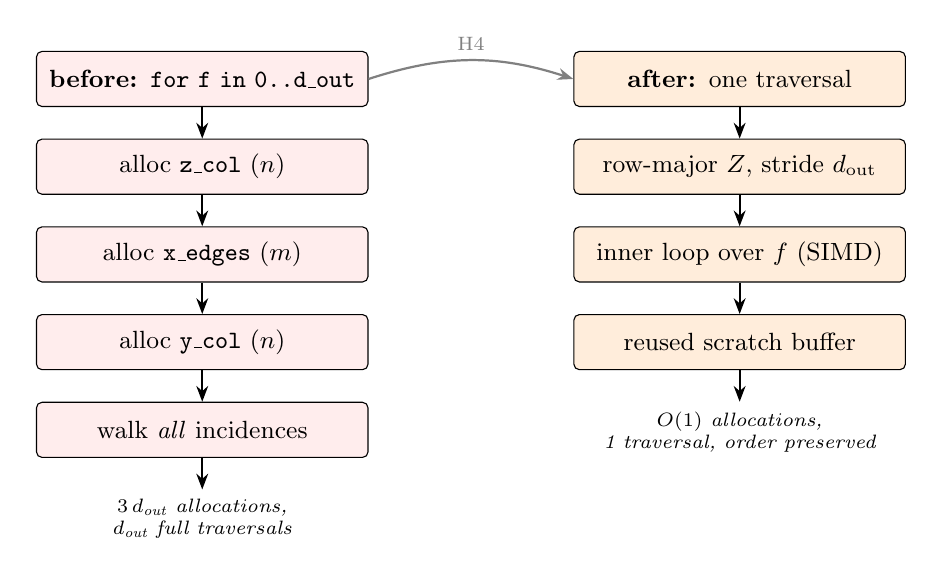
\begin{tikzpicture}[
  font=\small,
  box/.style={draw, rounded corners=2pt, align=center, inner sep=3pt,
              minimum height=7mm, text width=40mm},
  old/.style={box, fill=red!7},
  new/.style={box, fill=orange!14},
  flow/.style={-{Stealth[length=2mm]}, thick},
  node distance=4mm
]

\node[old] (o1) {\textbf{before:} \texttt{for f in 0..d\_out}};
\node[old, below=of o1] (o2) {alloc \texttt{z\_col} ($n$)};
\node[old, below=of o2] (o3) {alloc \texttt{x\_edges} ($m$)};
\node[old, below=of o3] (o4) {alloc \texttt{y\_col} ($n$)};
\node[old, below=of o4] (o5) {walk \emph{all} incidences};
\node[below=of o5, font=\scriptsize\itshape, text width=42mm, align=center]
  (o6) {$3\,d_{\text{out}}$ allocations,\\$d_{\text{out}}$ full traversals};

\draw[flow] (o1) -- (o2); \draw[flow] (o2) -- (o3);
\draw[flow] (o3) -- (o4); \draw[flow] (o4) -- (o5);
\draw[flow] (o5) -- (o6);

\node[new, right=26mm of o1] (n1) {\textbf{after:} one traversal};
\node[new, below=of n1] (n2) {row-major $Z$, stride $d_{\text{out}}$};
\node[new, below=of n2] (n3) {inner loop over $f$ (SIMD)};
\node[new, below=of n3] (n4) {reused scratch buffer};
\node[below=of n4, font=\scriptsize\itshape, text width=42mm, align=center]
  (n5) {$O(1)$ allocations,\\1 traversal, order preserved};

\draw[flow] (n1) -- (n2); \draw[flow] (n2) -- (n3);
\draw[flow] (n3) -- (n4); \draw[flow] (n4) -- (n5);

\draw[flow, gray] (o1.east) to[bend left=18] node[above,font=\scriptsize]{H4} (n1.west);

\end{tikzpicture}
\caption{Hypothesis H4: the convolution forward passes re-walk the entire
incidence structure once per output feature and allocate three temporaries
each time. Blocking the feature loop \emph{inside} the traversal keeps the
per-element summation order (and hence the numerics) but turns
$d_{\text{out}}$ traversals into one. The expected gain grows with
$d_{\text{out}}$ --- which is what the \texttt{feature\_dim} $\in
\{1,8,32,128\}$ sweep is designed to confirm or refute.}
\end{figure}


\end{document}
